% !TEX program = xelatex

\documentclass{resume}
\usepackage{graphicx}
\usepackage{tabularx}
\usepackage{tabu}
\usepackage{multirow}
\usepackage{progressbar}
% \usepackage{zh_CN-Adobefonts_external} % Simplified Chinese Support using external fonts (./fonts/zh_CN-Adobe/)
\usepackage{zh_CN-Adobefonts_internal} % Simplified Chinese Support using system fonts


\begin{document}
\pagenumbering{gobble} % suppress displaying page number

% {
% % change Large font here
% \Large{
%   \begin{tabu}{ c l r }
%    \multirow{5}{1in}{\includegraphics[width=0.88in]{avatar}} & \scshape{Bin Yuan} & {Python~}\progressbar{0.75} \\
%     & \email{yuanbin2014@gmail.com} & {Scala~}\progressbar{0.5} \\
%     & \phone{(+86) 131-221-87xxx} & {Linux~}\progressbar{0.7} \\
%     & \linkedin[billryan8]{https://www.linkedin.com/in/billryan8} & {Flask~}\progressbar{0.5} \\
%     & \github[github.com/billryan]{https://github.com/billryan} & {Javascript~}\progressbar{0.5}
%   \end{tabu}
% }
% }

% {
% % change Large font here
% \Large{
%   \begin{tabu}{ c l }
%    \multirow{4}{1in}{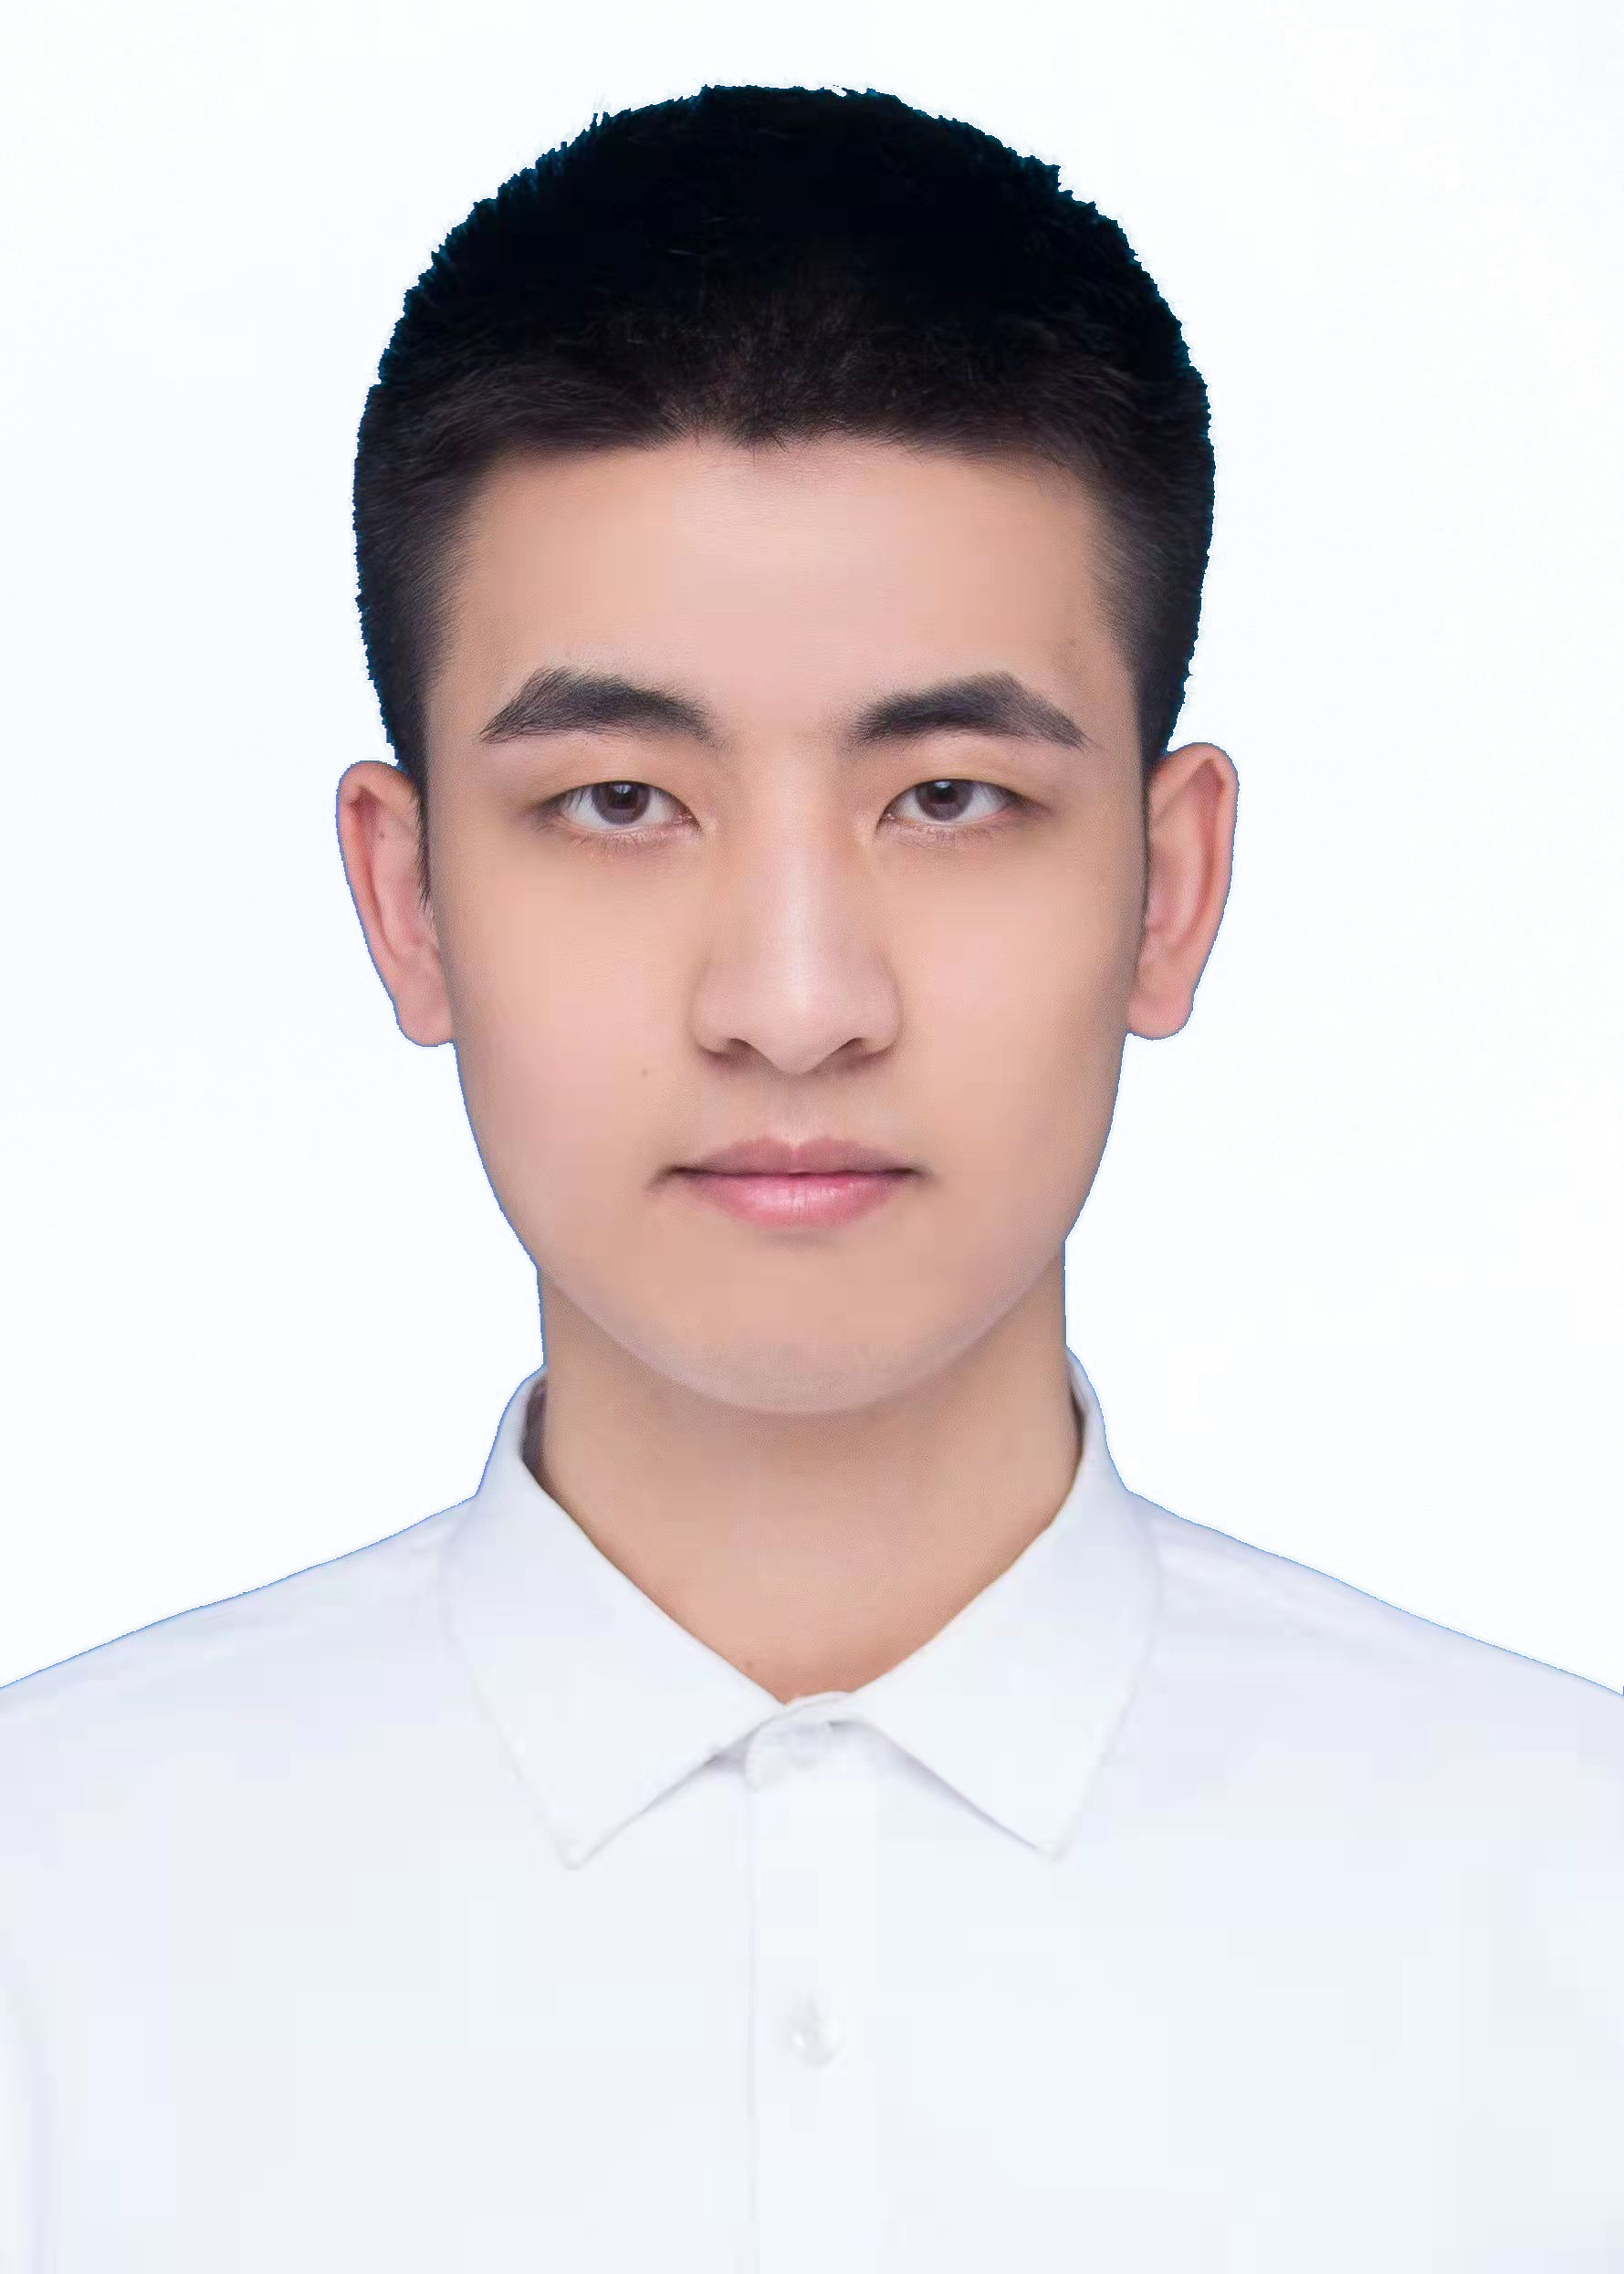
\includegraphics[width=0.88in]{lzj_avatar}} & \scshape{Zujing Liu} \\
%     & \email{zujing.liu@whu.edu.cn} \\
%     & \phone{(+86) 187-9005-5889} \\
%     & \homepage[liuxiaozhu.github.io]{https://liuxiaozhu01.github.io/} \\
%     & \github[github.com/liuxiaozhu01]{https://github.com/liuxiaozhu01} 
%   \end{tabu}
% }
% }

{
% change Large font here
\Large{
  \begin{tabularx}{\textwidth}{@{} c X r @{}}
   \multirow{4}{1in}[1.em]{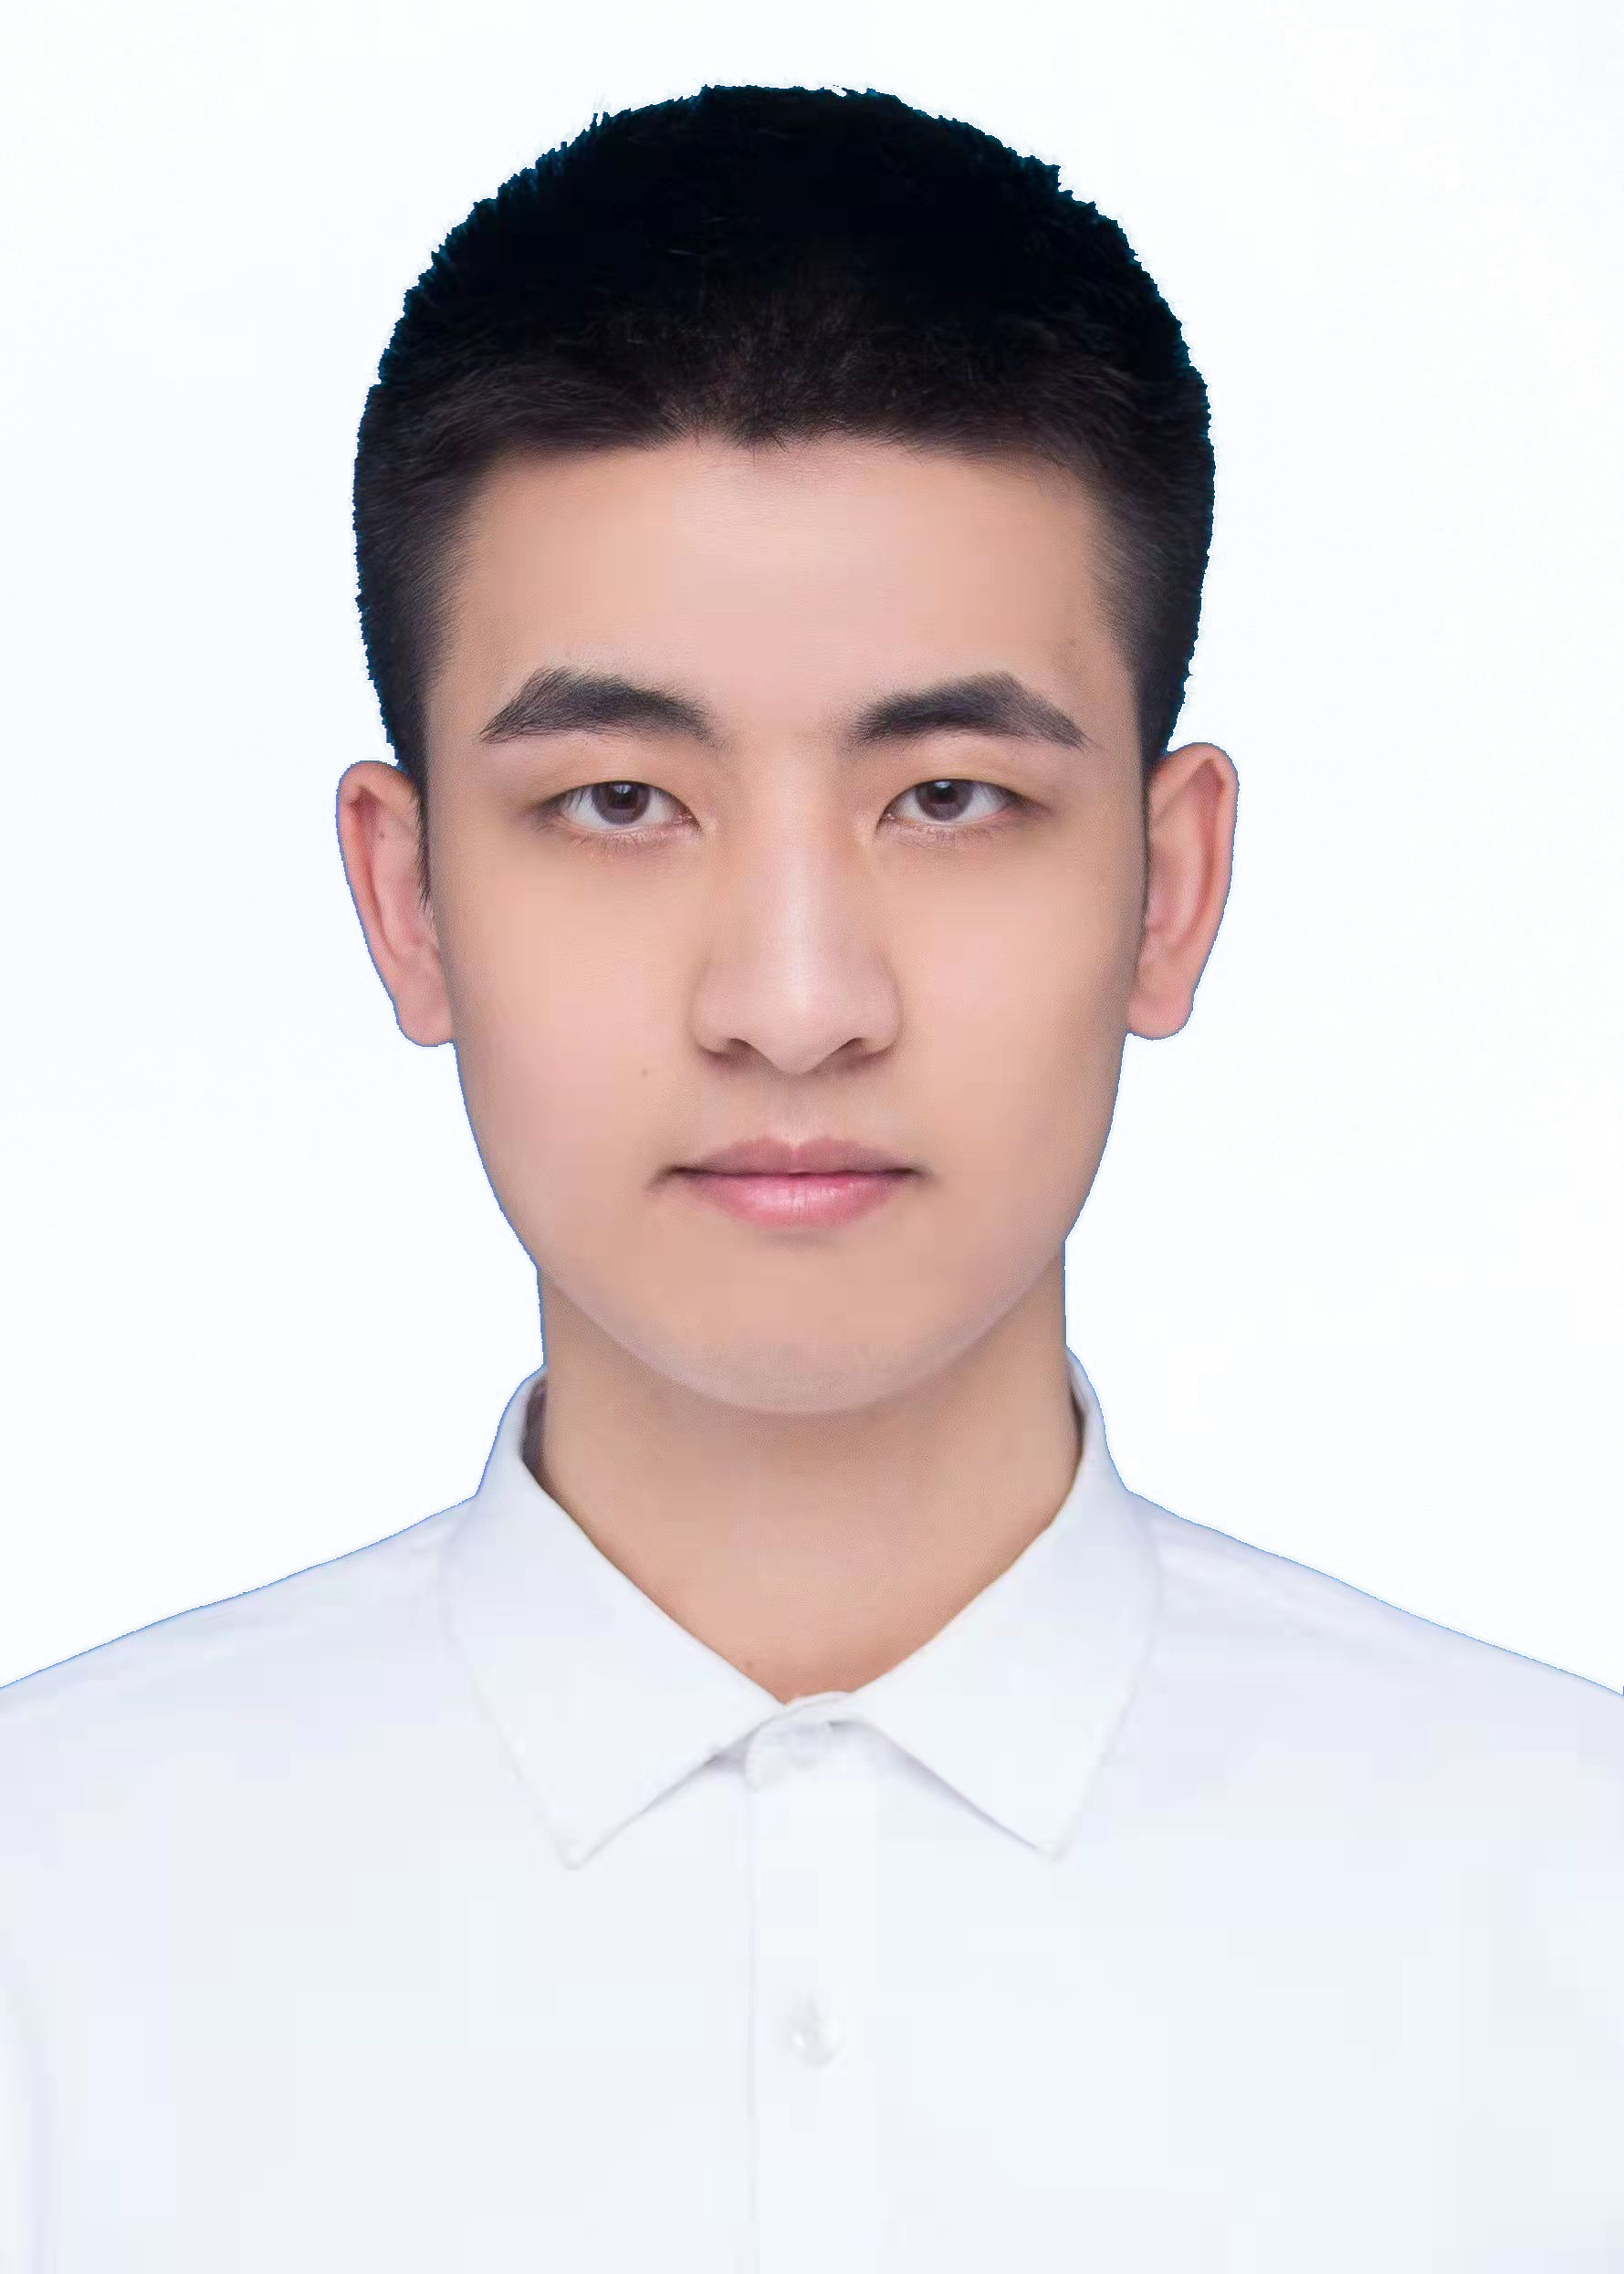
\includegraphics[width=0.88in]{lzj_avatar}} & \textbf{刘祖靖} & \email{zujing.liu@whu.edu.cn} \\
    & 武汉大学\ 计算机学院 & \phone{(+86) 187-9005-5889} \\
    & 计算机科学与技术 & \homepage[liuxiaozhu.github.io]{https://liuxiaozhu01.github.io/} \\
    &                  & % \github[github.com/liuxiaozhu01]{https://github.com/liuxiaozhu01} 
  \end{tabularx}
}
}

% \section{\faUser\ 个人总结}
% 本科综合排名Top14\%(珠峰计划内)获武汉大学荣誉学位,科研成果获\textcolor{red}{已授权发明专利}一项;硕士期间以\textcolor{red}{第一作者发表论文},研究成果在投。热爱技术研究,兼具独立攻关能力与高效团队协作精神。

% % 研究兴趣部分
% \noindent
% \textbf{研究兴趣}:
% \begin{itemize}[nosep, leftmargin=*, topsep=0pt, partopsep=0pt]
%       \item 模型轻量化:\textit{结构化剪枝、知识蒸馏、低比特量化}\ \ 推理加速:\textit{KV缓存优化、隐式CoT推理}
%       % \item 推理加速:KV缓存优化、隐式CoT推理、轻量化部署
% \end{itemize}

\vspace{-1mm}
\section{\faGraduationCap\ 教育经历}
\datedsubsection{\textbf{武汉大学}}{2023.09 -- 2026.07}
\textit{学术型硕士(推免)}————计算机科学与技术————导师夏桂松(杰青,教授)、高源(副教授)
% \datedsubsection{计算机学院-计算机科学与技术-导师夏桂松(杰青,教授)、高源(副教授)}{\textit{学术型硕士(推免)}}
\vspace{-2mm}
\datedsubsection{\textbf{武汉大学}}{2019.09 -- 2023.07}
\textit{学士(\textcolor{red}{珠峰计划})} ————计算机科学与技术(弘毅班)\textsuperscript{\dag}————GPA 3.81/4.00, Top14\%
% \datedsubsection{计算机学院-计算机科学与技术(弘毅班)-GPA3.81/4.00, Top14\% }{\textit{学士(荣誉学位)}}

% 计算机学院弘毅班为原弘毅学堂计算机方向荣誉计划调整来的精英班级,弘毅学堂授毕业生「荣誉学位」认证拔尖背景。
% {\footnotesize  \dag 由弘毅学堂(国家珠峰计划拔尖基地)计算机荣誉计划调整而来,培养计算机领域拔尖人才并授予「荣誉学位」。​}

% {\footnotesize  \dag 系国家基础学科拔尖学生培养试验计划(珠峰计划),由武汉大学计算机学院精英化培养并授予「荣誉学位」。​}
{\footnotesize  \dag 系国家基础学科拔尖学生培养试验计划(珠峰计划),由武汉大学计算机学院精英化、个性化独立培养。​}
% {\scriptsize  * 计算机学院弘毅班为原弘毅学堂计算机方向荣誉计划调整而来,弘毅学堂授毕业生「荣誉学位」认证拔尖背景。\\
% \dag 弘毅学堂为武汉大学荣誉学院,是响应国家基础学科拔尖学生培养试验计划(珠峰计划)所办的创新型拔尖人才培养基地}


%%%%%%%%%%%%%%%%%%%%%%%%%%%%%%%%%%% 专业技能 %%%%%%%%%%%%%%%%%%%%%%%%%%%%%%%%%%%
% \vspace{-1mm}
% \section{\faCogs\ 技术能力}
% \begin{tabularx}{\textwidth}{@{} >{\raggedright}X >{\raggedright}X @{}}
%   % 左列
%   \textbf{编程语言}: 
%     \begin{itemize}[nosep, leftmargin=*, topsep=0pt, partopsep=0pt]
%       \item Python > Shell > C/C++ > Java
%     \end{itemize}
%   &
%   % 右列
%   \textbf{平台框架}: 
%     \begin{itemize}[nosep, leftmargin=*, topsep=0pt, partopsep=0pt]
%       \item PyTorch, \LaTeX, \faLinux Linux, \faGit, VSCode
%     \end{itemize}
% \end{tabularx}

% \vspace{-3mm}

% % 研究兴趣部分
% \noindent
% \textbf{研究兴趣}:
% \begin{itemize}[nosep, leftmargin=*, topsep=0pt, partopsep=0pt]
%       \item 模型压缩:\textit{结构化剪枝、知识蒸馏、低比特量化}\ \ 推理加速:\textit{KV缓存优化、隐式CoT推理}
%       % \item 推理加速:KV缓存优化、隐式CoT推理、轻量化部署
% \end{itemize}

\vspace{-1mm}
\section{\faCogs\ 技术能力}
% \noindent
% \textbf{系统开发}: 
\subsection{\textbf{系统开发:}}
\begin{itemize}[nosep, leftmargin=*, topsep=0pt, partopsep=0pt]
    \item 熟悉Linux系统开发环境,熟练使用Git/GCC等开发工具链以及Shell/Python自动化脚本。
    \item 熟悉PyTorch开发框架和LLM工具链HuggingFace Transformers,了解CUDA并行编程。
    % \item 掌握PyTorch框架下工程化实践,熟悉HuggingFace Transformers开发,了解CUDA并行编程。
\end{itemize}

\vspace{-2mm}

% 研究兴趣部分
\noindent
\subsection{\textbf{研究兴趣:}}
\begin{itemize}[nosep, leftmargin=*, topsep=0pt, partopsep=0pt]
      \item 模型压缩:\textit{结构化剪枝、知识蒸馏、低比特量化}\ \ 推理加速:\textit{KV缓存优化、隐式CoT推理}
      % \item 推理加速:KV缓存优化、隐式CoT推理、轻量化部署
\end{itemize}


%%%%%%%%%%%%%%%%%%%%%%%%%%%%%%% 项目经历 %%%%%%%%%%%%%%%%%%%%%%%%%%%%%%%%%
\vspace{-1mm}
\section{\faTasks\ 项目经历}
\datedsubsection{\textbf{大模型轻量化与高效推理关键技术研究}}{2024.03 -- 至今}  % 这个是编的
\begin{itemize}
  % \item 研发一种应用于低计算资源平台的,基于优化的大模型结构化剪枝方法。产出一篇论文成果在投。
  % \item 提出轻量化部署的策略梯度优化剪枝框架,实现消费级GPU大模型高效压缩(ACL在投)。
  \item 提出消费级GPU大模型轻量化部署的策略梯度优化剪枝框架,\textcolor{red}{产出一篇论文成果}。
  % \item 探索思维链 (CoT) 压缩/隐式思维链推理方法,旨在提高大模型推理速度。
  \item 研究推理过程中动态压缩KV缓存的方法,提高推理速度,缓解KV缓存膨胀问题。
  \item 研究通过隐式/显式思维链对比蒸馏方法,实现隐式思维链的可解释性推理。
\end{itemize}

\datedsubsection{\textbf{基于大模型的商品属性智能解析系统}}{2023.04 -- 2023.08}
\begin{itemize}
  \item 运用大模型技术,深度解析商品描述,实现商品属性智能标注与分类。
  % 实现真实室内情景实时模拟,提供自由视角与对象跟踪等可操作功能。
  \item 担任团队负责人,搭建商品属性自动标注框架;利用P-Tuning v2对预训练ChatGLM-6B微调。
  \item \textbf{神州控股第三届校园极客大赛},入围\textcolor{red}{总决赛(13/300+)},获得\textcolor{red}{优胜奖}。
\end{itemize}

% \vspace{-3mm}

\datedsubsection{\textbf{智能可信辨识技术及在城市安全领域的应用}}{2020.09 -- 2021.08}
% 湖北省技术创新专项(重大项目)
\begin{itemize}
  \item 开发室内场景 3D 行人仿真模块,实现实时渲染与动态目标追踪,支持自由视点交互操作。
  % 实现真实室内情景实时模拟,提供自由视角与对象跟踪等可操作功能。
  \item 主导视频展示模块,设计实现 “流水线式视频处理分析框架”,视频处理分析延迟降低60\%。
  \item 提出 “视频流帧率调整方法、装置、设备及可读存储介质”,现\textcolor{red}{已获得发明专利授权}。% 解决视频帧率波动与缺失帧问题,(专利号:ZL 2021 1 1639965.1)
\end{itemize}

\vspace{-3mm}
\section{\faSearch\ 科研经历}
\datedsubsection{\textbf{Bypass Back-propagation: Optimization-based Structural Pruning for Large Language Models via Policy Gradient}}{ACL 投稿(第一作者)}
% \role{Summer Intern}{Manager: xxx}
% Brief introduction: xxx.
\begin{itemize}
  \item 一种\textbf{基于优化的 LLM 结构化剪枝方法},直接以模型损失为剪枝优化目标。
  \item 使用伯努利分布对剪枝掩码进行概率化建模,通过策略梯度估计器优化概率参数,\textbf{避免反向传播}。
  \item 与现有的启发式剪枝技术相比,性能更优越,并兼顾计算高效性。
\end{itemize}

% \vspace{-3mm}
% \section{\faUsers\ 学生工作}
% \datedsubsection{\textbf{计算机学院2023级硕士1班}  \quad \textit{团支部书记}}{2023 -- 至今}
% \begin{itemize}
%   \item 负责班级团支部工作,组织开展多项团日活动,提升班级凝聚力。
%   % \item 对接学院团委,积极参与学院团委党委组织的各项活动。
% \end{itemize}

% \vspace{-3mm}

% \datedsubsection{\textbf{武汉大学心理卫生健康协会}  \quad \textit{新闻部部长}}{2020 -- 2021}
% \begin{itemize}
%   \item 撰写的多篇新闻稿件发表于武汉大学新闻网、极目新闻等平台,并被多家媒体转载。
%   % \item 负责协会新闻稿件的撰写、编辑、发布工作,提升协会的社会影响力。
% \end{itemize}

\vspace{-3mm}
\section{\faTrophy\ 荣誉奖项}
\datedsubsection{本科阶段}{2019 -- 2023}
\begin{itemize}[parsep=0.5ex]
  \item \textbf{奖学金}: 武汉大学乙等学业奖学金(Top 10\%),国家励志奖学金(Top 15\%)
  \item \textbf{荣誉}:武汉大学优秀学生(Top 10\%),优秀共青团员(2020-2022)
\end{itemize}

%% Reference
%\newpage
%\bibliographystyle{IEEETran}
%\bibliography{mycite}
\end{document}
